\begin{theorem} (Дифференцирование несобственного интеграла Римана, зависящего от параметра)
	Пусть дана $f \in C(\lsi{a; b} \times [c; d])$ и выполнены следующие условия:
	\begin{enumerate}
		\item $\pd{f}{y}(x, y) \in C(\lsi{a; b} \times [c; d])$
		
		\item $\int_a^b \pd{f}{y}(x, y)dx$ сходится равномерно на $[c; d]$
		
		\item Существует $y_0 \in [c; d]$ такой, что $\int_a^b f(x, y_0)dx$ сходится
	\end{enumerate}
	Тогда функция $I(y) = \int_a^b f(x, y)dx$ дифференцируема на $[c; d]$ и верна формула:
	\[
		\frac{dI}{dy}(y) = \frac{d}{dy}\ps{\int_a^b f(x, y)dx} = \int_a^b \pd{f}{y}(x, y)dx
	\]
\end{theorem}

\begin{proof}
	 Для начала отметим, что $f(x, t)$ можно представить следующим образом:
	 \[
	 	f(x, t) = f(x, y_0) + \int_{y_0}^t \pd{f}{y}(x, y)dy
	 \]
	 По условию интеграл по производной сходится равномерно. Стало быть, применима теорема об интегрировании собственного интеграла Римана, зависящего от параметра:
	 \[
	 	\int_{y_0}^t \ps{\int_a^b \pd{f}{y}(x, y)dx}dy = \int_a^b \ps{\int_{y_0}^t \pd{f}{y}(x, y)dy}dx \text{ --- сходятся}
	 \]
	 Осталось проинтегрировать равенство с $f$. Это будет корректно, потому что в правой части оба интеграла сойдутся:
	 \[
	 	I(t) = \int_a^b f(x, t)dx = \int_a^b f(x, y_0)dx + \int_{y_0}^t \ps{\int_a^b \pd{f}{y}(x, y)dx}dy
	 \]
	 По следствию \ref{parametrized_integral_continuity} внутренний интеграл справа является непрерывной функцией. Значит, по теореме об основных свойствах интеграла Римана с переменным верхним пределом заключаем, что $I(t)$ дифференцируема на $[c; d]$ и верно требуемое равенство:
	\[
		\pd{I}{y}(t) = \int_a^b \pd{f}{y}(x, t)dx
	\]
\end{proof}

\begin{example} (Интеграл Дирихле)
	Покажем справедливость следующего равенства при $\alpha = 1$:
	\[
		\int_0^{+\infty} \frac{\sin(\alpha x)}{x}dx = \frac{\pi}{2} \cdot \sgn(\alpha)
	\]
	Идея следующая: рассмотрим $F(y)$, для которой значение нашего интеграла есть $F(0)$. Вычислим $F$ через нахождение производной, решим задачу Коши и тривиально получим ответ.
	
	Итак, рассмотрим следующую $F$:
	\[
		F(y) = \int_0^{+\infty} \frac{\sin(x)}{x}e^{-xy}dx
	\]
	По признаку Абеля, $F(y)$ сходится равномерно на $\lsi{0; +\infty}$:
	\begin{enumerate}
		\item $\int_0^{+\infty} \frac{\sin x}{x}dx$ сходится равномерно по $y \in \lsi{0; +\infty}$
		
		\item $e^{-xy}$ монотонна при любом $y$
		
		\item $e^{-xy}$ равномерно ограничена на $\lsi{0; +\infty} \times \lsi{0; +\infty}$
	\end{enumerate}
	Стало быть, можем воспользоваться теоремой о предельном переходе и получить, что $\lim_{y \to +\infty} F(y) = 0$. Посчитаем производную подыинтегральной функции  по параметру:
	\[
		\pd{}{y}\ps{\frac{\sin x}{x}e^{-xy}} = -\sin(x)e^{-xy}
	\]
	Несложно понять, что мы выполнили условия теоремы о дифференцировании:
	\begin{enumerate}
		\item $\sin(x)e^{-xy} \in C(\lsi{0; +\infty} \times \lsi{0; +\infty})$
		
		\item[2-3.] $\exists c > 0 \such \forall x \in \lsi{0; +\infty}\ \forall y \in \lsi{y_0; +\infty}\ \ |\sin x e^{-xy}| \le e^{-xy_0}$
	\end{enumerate}
	Коль скоро это так, верна цепочка равенств:
	\begin{multline*}
		F'(y) = -\int_0^{+\infty} \sin(x)e^{-xy}dx =
		\\
		\cos(x)e^{-xy}\Big|_0^{+\infty} + y\int_0^{+\infty} \cos(x)e^{-xy}dx =
		\\
		-1 + y\sin(x)e^{-xy}\Big|_0^{+\infty} + y^2\int_0^{+\infty} \sin(x)e^{-xy}dx
	\end{multline*}
	Таким образом, $F'(y) = \frac{-1}{1 + y^2}$, то есть $F(y) = C - \arctg y$. В силу условия $\lim_{y \to +\infty} F(y) = 0$ получаем итоговый результат:
	\[
		F(y) = \frac{\pi}{2} - \arctg y \Lora \int_0^{+\infty} \frac{\sin x}{x}dx = F(0) = \frac{\pi}{2}
	\]
\end{example}

\begin{example} (Интегралы Лапласа)
	Докажем формулы \textit{интегралов Лапласа}:
	\[
		I(\alpha) = \int_0^{+\infty} \frac{\cos(\alpha x)}{1 + x^2}dx = \frac{\pi}{2}e^{-|\alpha|}; \quad K(\alpha) = \int_0^{+\infty} \frac{x\sin(\alpha x)}{1 + x^2}dx = \frac{\pi}{2}e^{-|\alpha|}\sgn(\alpha)
	\]
	Не умаляя общности, разберёмся только с $I(\alpha)$. Для начала, покажем равномерную сходимость этого интеграла на $\R$:
	\[
		\md{\frac{\cos(\alpha x)}{1 + x^2}} \le \frac{1}{1 + x^2}
	\]
	В силу оценки, всё доказано по признаку Вейерштрасса. Далее мы хотим точно так же, как и ранее вычислить $I(\alpha)$ через диффура (без ограничений рассмотрим $\alpha > 0$), поэтому нужно проверить условия теоремы о дифференцировании:
	\begin{enumerate}
		\item $\ps{\frac{\cos(\alpha x)}{1 + x^2}}'_\alpha = \frac{-x\sin(\alpha x)}{1 + x^2} \in C(\lsi{0; +\infty} \times \R)$
		
		\item $\int_0^{+\infty} \ps{-\frac{x\sin(\alpha x)}{1 + x^2}} = -K(\alpha)$ сходится равномерно на $\R$
		
		\item При $\alpha = 0$ интеграл сходится
	\end{enumerate}
	Стало быть, можно записать равенство $I'(\alpha) = -K(\alpha)$. Осталось провернуть следующий трюк (по-хорошему, взятие ещё одной производной надо обосновывать, но после первого раза это, думаю, понятно как сделать):
	\[
		\ps{\frac{\pi}{2} + I'(\alpha)}' = I''(\alpha); \quad \frac{\pi}{2} + I'(\alpha) = \int_0^{+\infty} \ps{\frac{\sin(\alpha x)}{x} - \frac{x\sin(\alpha x)}{1 + x^2}}dx = \int_0^{+\infty} \frac{\cos(\alpha x)}{1 + x^2}dx
	\]
	Несложно заметить, что последний интеграл есть просто исходный $I(\alpha)$. Стало быть, мы получили диффур $I''(\alpha) = I(\alpha)$, общее решение которого имеет вид $I(\alpha) = C_1e^{\alpha} + C_2e^{-\alpha}$. Осталось решить задачу Коши:
	\begin{itemize}
		\item $|I(\alpha)| \le \int_0^{+\infty} \frac{dx}{1 + x^2} = \frac{\pi}{2}$, то есть $C_1 = 0$ в силу ограниченности
		
		\item $I(0) = \pi / 2 = C_2$
	\end{itemize}
	Итого, $I(\alpha) = \frac{\pi}{2}e^{-\alpha}$ при $\alpha > 0$. Аналогично доказывается формула при $\alpha < 0$, а $K(\alpha)$ можно вообще получить как производную от $I(\alpha)$
\end{example}

\subsection{Эйлеровы интегралы}

\begin{definition}
	\textit{Гамма-функцией} называется следующая функция:
	\[
		\Gamma(\alpha) = \int_0^{+\infty} x^{\alpha - 1}e^{-x}dx,\ \alpha > 0
	\]
\end{definition}

\begin{proposition}
	Гамма-функция сходится равномерно на любом отрезке внутри луча $(0; +\infty)$
\end{proposition}

\begin{proof}
	Рассмотрим $\alpha \in [\alpha_0; \alpha_1] \subset (0; +\infty)$. Так как степенная функция категорически меняет свое поведение при переходе $x = 1$, то мы разобьём интеграл на 2 и оценим каждую часть по отдельности:
	\[
		\int_0^{+\infty} x^{\alpha - 1}e^{-x}dx = \int_0^1 x^{\alpha - 1}e^{-x}dx + \int_1^{+\infty} x^{\alpha - 1}e^{-x}dx
	\]
	\begin{enumerate}
		\item \(\forall x \in [0; 1]\ \ x^{\alpha - 1}e^{-x} \le x^{\alpha_0 - 1} \cdot 1 = x^{\alpha_0 - 1}\)
		
		\item \(\forall x \ge 1\ \ x^{\alpha - 1}e^{-x} \le x^{\alpha_1 - 1}e^{-x}\)
		
		\item Дополнительно заметим, что экспонента на луче всегда перебивает степенную функцию:
		\[
			\exists x_0 \in \lsi{1; +\infty}, C > 0 \such \forall x \ge x_0\ \ x^{\alpha_1 - 1}e^{-x} \le Ce^{-x / 2}
		\]
	\end{enumerate}
	Итого, мы умеем ограничивать интеграл для произвольного $\alpha$ из отрезка при помощи значений на концах отрезка:
	\begin{multline*}
		\int_0^{+\infty} x^{\alpha - 1}e^{-x}dx = \int_0^1 x^{\alpha - 1}e^{-x}dx + \int_1^{+\infty}x^{\alpha - 1}e^{-x}dx \le
		\\
		\int_0^1 x^{\alpha_0 - 1}dx + \int_1^{x_0} x^{\alpha_1 - 1}e^{-x}dx + \int_{x_0}^{+\infty} Ce^{-x / 2}dx
	\end{multline*}
	Каждый интеграл не зависит от $\alpha$ и сходится. Стало быть, гамма-функция сходится равномерно на отрезке.
\end{proof}

\begin{theorem} (Основные свойства гамма-функции)
	\begin{enumerate}
		\item Гамма-функция относится к классу бесконечно дифференцируемых на $(0; +\infty)$
		
		\item (Формула понижения) $\Gamma(\alpha + 1) = \alpha\Gamma(\alpha),\ \alpha > 0$
		
		\item (Продолжение факториала) $\forall n \in \N_0\ \ \Gamma(n + 1) = n!$
	\end{enumerate}
\end{theorem}

\begin{proof}~
	\begin{enumerate}
		\item Проверим условия теоремы о дифференцировании:
		\begin{enumerate}
			\item $x^{\alpha - 1} \cdot \ln(x) \cdot e^{-x} \in C\big((0; +\infty) \times (0; +\infty)\big)$
			
			\item Интеграл от производной тоже должен сходиться равномерно на любом отрезке в луче $(0; +\infty)$. Доказательство почти повторяет то, что происходило для гамма-функции, только нужно учесть простую оценку на натуральный логарифм:
			\[
				\forall x \in (0; +\infty)\ \ \ln(x) \le \sqrt{x} = x^{1 / 2}
			\]
			
			\item При $\alpha = 1$ есть тривиальная сходимость
		\end{enumerate}
		Стало быть, производная интеграла существует и определяется известной формулой. Из правила дифференцирования следует, что картина не меняется при взятии производной высшего порядка, то есть гамма-функция бесконечно дифференцируема
		
		\item Нужно просто взять интеграл $\Gamma(\alpha + 1)$ по частям:
		\[
			\Gamma(\alpha + 1) = \int_0^{+\infty} x^\alpha e^{-x}dx = -x^\alpha e^{-x}\Big|_0^{+\infty} + \alpha \int_0^{+\infty} x^{\alpha - 1}e^{-x}dx = \alpha\Gamma(\alpha)
		\]
		
		\item Доказывается индукцией по $n$:
		\begin{itemize}
			\item База $n = 0$: $\Gamma(1) = \int_0^{+\infty} e^{-x}dx = 1 = 0!$
			
			\item Переход $n > 0$: пользуемся формулой понижения
		\end{itemize}
	\end{enumerate}
\end{proof}

\begin{definition}
	\textit{Бета-функцией} называется следующая функция двух аргументов:
	\[
		\forall \alpha, \beta > 0\ \ B(\alpha, \beta) := \int_0^1 x^{\alpha - 1}(1 - x)^{\beta - 1}dx
	\]
\end{definition}

\begin{proposition}
	Бета-функция сходится равномерно на любом прямоугольнике из $(0; +\infty) \times (0; +\infty)$
\end{proposition}

\begin{theorem} (Связь бета- и гамма-функций)
	Имеет место равенство:
	\[
		\forall \alpha, \beta > 0\ \ B(\alpha, \beta) = \frac{\Gamma(\alpha) \cdot \Gamma(\beta)}{\Gamma(\alpha + \beta)}
	\]
\end{theorem}

\begin{proof}
	На самом деле покажем равенство $B(\alpha, \beta) \cdot \Gamma(\alpha + \beta) = \Gamma(\alpha) \cdot \Gamma(\beta)$. Коль скоро бета- и гамма-функции есть несвязанные интегралы, то их произведение можно записать как повторный (а равно и двойной, поскольку подынтегральные функции неотрицательные):
	\[
		B(\alpha, \beta) \cdot \Gamma(\alpha + \beta) = \int_0^1 \int_0^{+\infty} x^{\alpha - 1}(1 - x)^{\beta - 1}y^{\alpha + \beta - 1}e^{-y}dydx
	\]
	Далее идея состоит в том, чтобы применить замену переменных $(x, y) = (\xi / (\xi + \eta), \xi + \eta)$, которая является взаимно однозначной ($(\xi, \eta) = (xy, (1 - x)y)$). При этом множество, по которому берётся интеграл, неограничено, и надо придумать, чем мы будем его исчерпывать. Например, возьмём  квадрат, который с полосы в плоскости $xoy$ переходит в трапецию, чьи боковые стороны лежат на осях $o\xi$ и $o\eta$:
	\begin{center}
		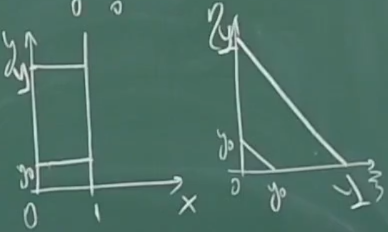
\includegraphics[width=0.4\textwidth]{images/beta_function.png}
	\end{center}
	
	Посчитаем Якобиан:
	\[
		\pd{(\xi, \eta)}{(x, y)} = \Det{
			y& &x
			\\
			-y& &1 - x
		} = y - xy + xy = y > 0
	\]
	И применим теорему о замене переменной в интеграле:
	\begin{multline*}
		\Gamma(\alpha) \cdot \Gamma(\beta) = \int_0^{+\infty} \int_0^{+\infty} \xi^{\alpha - 1} \eta^{\beta - 1} e^{-(\xi + \eta)}d\eta d\xi =
		\\
		\int_0^1 \int_0^{+\infty} x^{\alpha - 1} y^{\alpha - 1} (1 - x)^{\beta - 1} y^{\beta - 1} e^{-y} \cdot ydydx =
		\\
		\int_0^1 \int_0^{+\infty} x^{\alpha - 1} y^{\alpha + \beta - 1} (1 - x)^{\beta - 1} e^{-y} dydx = B(\alpha, \beta) \cdot \Gamma(\alpha + \beta)
	\end{multline*}
\end{proof}

\begin{theorem} (Формула Гаусса-Эйлера)
	Имеет место следующее равенство:
	\[
		\forall \alpha > 0\ \ \Gamma(\alpha) = \lim_{n \to \infty} n^\alpha \frac{(n - 1)!}{\alpha(\alpha + 1) \cdot \ldots \cdot (\alpha + n - 1)}
	\]
\end{theorem}

\begin{proof}
	Произведём разбор случаев:
	\begin{itemize}
		\item $\alpha \ge 1$. Сперва перепишем гамма-функцию в её каноническом виде (почти в таком виде её рассматривал Лежандр):
		\[
			\Gamma(\alpha) = \int_0^{+\infty} x^{\alpha - 1}e^{-x}dx = \{x = \ln(1 / u)\} = \int_0^1 \ln^{\alpha - 1} \ps{\frac{1}{u}}du
		\]
		Идея состоит в том, чтобы записать этот интеграл по теореме Леви через функции $f_n(u) = n(1 - u^{1 / n}) \to \ln(1 / u),\ n \to \infty,\ u \in (0; 1)$, а затем расписать всё через бета-функцию. Сначала покажем монотонность $f_n$ по $n$. Для этого рассмотрим $g(t) = t(1 - u^{1 / t})$ и посчитаем её производную:
		\[
			g'(t) = 1 - u^{1 / t} + t\ps{-\ps{-\frac{1}{t^2}}u^{1 / t} \cdot \ln u} = 1 - u^{1 / t} + \frac{1}{t}u^{1 / t}\ln u
		\]
		Чтобы показать положительность этой производной при $u \in (0; 1)$, нам нужно рассмотреть эту функцию как функцию от $y = u^{1 / t}$. Тогда $\phi(y) = 1 - y + y\ln y$, а для неё уже производная проще (при этом $y \in (0; 1)$, ибо $t \ge 1$ и $u \in (0; 1)$):
		\[
			\phi'(y) = -1 + \ln y + 1 = \ln y < 0
		\]
		Стало быть, из-за условия $\phi(1) = 0$ получаем $\forall y \in (0; 1)\ \phi(y) > 0$, то есть и $g'(t) > 0$ при $t \in (0; 1)$, что и требовалось. Осталось показать, что $f_n(u)$ при каждом $u \in (0; 1)$ сходится к $\ln(1 / u)$. Сделаем это через $g(t)$:
		\begin{multline*}
			\lim_{t \to +\infty} g(t) = \lim_{t \to +\infty} t(1 - u^{1 / t}) = \lim_{t \to +\infty} \frac{1 - u^{1 / t}}{1 / t} = \{\text{неопределенность } 0 / 0\} =
			\\
			\lim_{t \to +\infty} \frac{\frac{1}{t^2}u^{1 / t}\ln u}{-\frac{1}{t^2}} = -\ln u \cdot \lim_{t \to +\infty} u^{1 / t} = \ln \frac{1}{u}
		\end{multline*}
		В силу $\alpha \ge 1$, мы сохраняем сходимость снизу при возведении в степень, поэтому осталось просто расписать интеграл гамма-функции через предел:
		\begin{multline*}
			\Gamma(\alpha) = \lim_{n \to \infty} \int_0^1 f_n^{\alpha - 1}(u)du = \lim_{n \to \infty} n^{\alpha - 1} \int_0^1 (1 - u^{1 / n})^{\alpha - 1}du = \{v = u^{1 / n}\} =
			\\
			\lim_{n \to \infty} n^{\alpha - 1} \int_0^1 (1 - v)^{\alpha - 1} \cdot nv^{n - 1}dv = \lim_{n \to \infty} n^\alpha \int_0^1 (1 - v)^{\alpha - 1}v^{n - 1}dv = \lim_{n \to \infty} n^\alpha B(n, \alpha) =
			\\
			\lim_{n \to \infty} n^\alpha \frac{\Gamma(n)\Gamma(\alpha)}{\Gamma(\alpha + n)} = \lim_{n \to \infty} n^\alpha\frac{(n - 1)! \cdot \Gamma(\alpha)}{(\alpha + n - 1) \cdot \ldots \cdot \alpha \cdot \Gamma(\alpha)}
		\end{multline*}
		
		\item $0 < \alpha < 1$. Тогда мы можем всё запросто свести к уже доказанному:
		\begin{multline*}
			\Gamma(\alpha) = \frac{\Gamma(\alpha + 1)}{\alpha} = \frac{1}{\alpha} \lim_{n \to \infty} n^{\alpha + 1} \frac{(n - 1)!}{(\alpha + 1) \cdot \ldots \cdot (\alpha + n)} =
			\\
			\lim_{n \to \infty} n^\alpha \frac{(n - 1)!}{\alpha(\alpha + 1) \cdot \ldots \cdot (\alpha + n - 1)} \cdot \frac{n}{\alpha + n}
		\end{multline*}
		Выделенная справа дробь стремится к единице, поэтому требуемое доказано
	\end{itemize}
\end{proof}